% !TeX program = pdflatex
% Roots That Are Always There -- the virtual roots of a real polynomial in Lean 4.
% Part of the reverse-formalization line (Mathlib gaps -> formalize). Companion of the
% Budan-Fourier and Sturm formalizations: the structural theory of virtual roots (the d
% continuous substitutes for the real roots), with the Rolle-type interlacing.
% Build: pdflatex virtual-roots-lean.tex (twice, for refs)
% Verified against the Lean source 2026-06-16 (lake env lean VirtualRoots.lean, exit 0;
% #print axioms VirtualRoots.vroots_interlacing / vroots_isChain / vroots_getElem_mem ->
% propext, Classical.choice, Quot.sound only). Toolchain godsil v4.30. Worked examples
% (x^2+1, x^3-x) re-checked in exact arithmetic.

\documentclass[11pt]{article}
\usepackage[T1]{fontenc}
\usepackage{lmodern}
\usepackage{amsmath,amssymb,amsthm,booktabs,graphicx,hyperref}
\usepackage{xurl}
\usepackage[table]{xcolor}
\definecolor{ggteal}{HTML}{1B6F8C}
\definecolor{ggband}{HTML}{DCE7EB}
\definecolor{ggamber}{HTML}{E08A1E}
\definecolor{ggplum}{HTML}{7B4B94}
\usepackage[margin=1in]{geometry}
\usepackage{microtype}
\usepackage{float}
\usepackage[most]{tcolorbox}
\usepackage{tikz}
\usetikzlibrary{arrows.meta,positioning}
\setlength{\emergencystretch}{2em}
\newtheorem{theorem}{Theorem}
\newtheorem{lemma}{Lemma}
\newtheorem{proposition}{Proposition}
\newtheorem{remark}{Remark}
\newcommand{\lean}[1]{\texttt{#1}}
\newcommand{\R}{\mathbb{R}}
\newcommand{\V}{\mathrm{V}}
\newcommand{\Rd}{\mathcal{R}}
\hypersetup{colorlinks=true,linkcolor=ggteal,citecolor=ggteal,urlcolor=ggteal}
\newtcbox{\keybox}{on line,boxrule=0.9pt,colframe=ggteal,colback=ggband!40,
  arc=3pt,left=8pt,right=8pt,top=5pt,bottom=5pt}
\newcommand{\keyeq}[1]{\begin{center}\keybox{$\displaystyle #1$}\end{center}}

\title{\bf Roots That Are Always There\\[4pt]
  \large\normalfont The virtual roots of a real polynomial, machine-checked in Lean~4}
\author{Carles Mar\'in\thanks{Formalized with the assistance of an AI system (Claude,
Anthropic); the mathematics is classical, and every claim, scope statement, and limitation is
the author's responsibility. The boundary of the contribution---in particular what is \emph{not}
yet formalized---is set out plainly in Section~\ref{sec:boundary}, and the Lean kernel, not the
assistant, is what certifies the proofs.}\\[3pt]
  \normalsize Independent researcher\\
  \normalsize \texttt{karlesmarin@gmail.com}}
\date{June 2026}

\begin{document}
\maketitle

\begin{abstract}
A real polynomial of degree $d$ may have fewer than $d$ real roots, but it always has exactly $d$
\emph{virtual roots}: continuous, semialgebraic substitutes
$\rho_{d,1}(p)\le\cdots\le\rho_{d,d}(p)$ that coincide with the real roots when these exist and
otherwise sit where the polynomial comes closest to vanishing. They were introduced by
Gonz\'alez-Vega, Lombardi and Mah\'e~\cite{glm} and are the natural carrier of the Budan--Fourier
count~\cite{coste}. I report a complete, \lean{sorry}-free formalization in Lean~4 over Mathlib of
their \emph{structural theory}: the recursive construction by a choice operator $\Rd_d$ that
minimises $|p|$ on each interval where $p'$ keeps a constant sign; the fundamental count, that there
are exactly $d$ of them (\lean{vroots\_length}); that they come out sorted and inside the bracketing
interval (\lean{vroots\_isChain}, \lean{vroots\_subset\_Icc}); that $\Rd_d$ returns an actual root
wherever $p$ has one (\lean{R\_eval\_eq\_zero\_of\_le\_zero\_le}); and the \emph{Rolle interlacing}
\[
  \rho_{d,r}(p)\ \le\ \rho_{d-1,r}(p')\ \le\ \rho_{d,r+1}(p),
\]
the statement that each virtual root of $p'$ is wedged between two consecutive virtual roots of $p$
(\lean{vroots\_interlacing}). To the best of my knowledge---based on searches in June~2026 of
Mathlib, the Coq \lean{mathcomp-real-closed} library, the Isabelle AFP, and HOL~Light
(Section~\ref{sec:boundary})---virtual roots had not been formalized in any interactive theorem
prover; this is their first development. What is deliberately \emph{not} here is the exact
Budan--Fourier count, that the number of virtual roots in $(a,b]$ equals the sign-variation drop
$\V(a)-\V(b)$: that theorem fuses this construction with a second, independent one (the
\lean{fourierVar} of the companion Budan--Fourier formalization~\cite{bflean}) and is the explicit
sequel, named honestly in Section~\ref{sec:boundary}. Every theorem here depends only on the three
standard axioms \lean{propext}, \lean{Classical.choice}, \lean{Quot.sound}.
\end{abstract}

\medskip
\noindent\emph{What you will find here.} A short guided tour, built as a string of beads: each
section ends with the question the next answers. The first asks what a virtual root \emph{is}, and
why there are always exactly $d$ of them (Section~\ref{sec:q1}); the second, how to build them so a
machine will accept the construction (Section~\ref{sec:q2}); the third, where the formalization
genuinely resists (Section~\ref{sec:q3}); the fourth, what the certified theory gives---the Rolle
interlacing, and the road to the exact count (Section~\ref{sec:q4}). The load-bearing lemmas are in
one table (Section~\ref{sec:blocks}); the honest limits, including the deferred count, are in
Section~\ref{sec:boundary}; and the close asks the questions worth carrying forward. If you read
only two things, read the interlacing (Theorem~\ref{thm:interlace}) and Figure~\ref{fig:fillin}.

\section{The question that begins it}\label{sec:intro}

\emph{History bead.} Budan~\cite{budan} and Fourier~\cite{fourier} could bound the number of real
roots of a polynomial in an interval by a difference of sign counts, but the bound is only an
inequality: the surplus, always even, is the price of the roots that fail to be real. For two
centuries that surplus was an error term. In 1998 Gonz\'alez-Vega, Lombardi and Mah\'e~\cite{glm}
turned it into an object. They observed
that a degree-$d$ polynomial, real-rooted or not, carries $d$ canonical real numbers---the
\emph{virtual roots}---that vary continuously with the coefficients, restrict to the genuine roots
when those are present, and account \emph{exactly} for the Budan--Fourier count. Coste, Lajous,
Lombardi and Roy later made the count an equality through them~\cite{coste}.

The picture to keep is the simplest non-trivial one. The polynomial $p=x^2+1$ has no real root, yet
its graph dips to a single closest approach at $x=0$. Virtual roots see that approach: $p$ has the
double virtual root $\rho_{2,1}=\rho_{2,2}=0$. Where a real root would be, there is a virtual one;
where two conjugate roots hide, the two virtual roots collide at the foot of the dip
(Figure~\ref{fig:fillin}). Nothing is invented---the construction is explicit and semialgebraic---and
nothing is lost: the count is always $d$.

This paper formalizes the part of that story that is structural: the construction, the count, the
order, and the interlacing. The arithmetic equality with the sign-variation drop---the part that
earns the name ``Budan--Fourier''---is the sequel, and Section~\ref{sec:boundary} says exactly why it
is held back. What begins it is the question: \emph{what is a virtual root, concretely enough that a
proof assistant will accept it, and why are there always $d$?}

\begin{figure}[htbp]
\centering
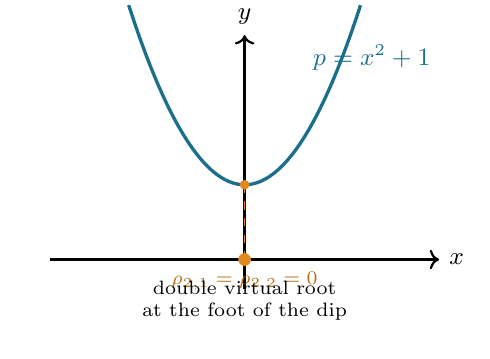
\begin{tikzpicture}[scale=0.95]
  \useasboundingbox (-2.9,-0.95) rectangle (2.9,3.1);
  % axes
  \draw[->,thick] (-2.6,0) -- (2.6,0) node[right,font=\small] {$x$};
  \draw[->,thick] (0,-0.4) -- (0,3.0) node[above,font=\small] {$y$};
  % parabola y = x^2 + 1 (scaled)
  \draw[ggteal,very thick,domain=-1.55:1.55,samples=80] plot (\x,{\x*\x+1});
  \node[ggteal,font=\small] at (1.7,2.7) {$p=x^2+1$};
  % minimum / double virtual root
  \filldraw[ggamber] (0,1) circle (1.6pt);
  \draw[ggamber,dashed] (0,1) -- (0,0);
  \filldraw[ggamber] (0,0) circle (2.2pt);
  \node[ggamber!80!black,font=\scriptsize,below=1pt] at (0,0)
    {$\rho_{2,1}=\rho_{2,2}=0$};
  \node[font=\scriptsize,align=center] at (0,-0.55) {double virtual root\\at the foot of the dip};
\end{tikzpicture}
\caption{Roots that are always there. The polynomial $x^2+1$ has \emph{no} real root, but a double
virtual root at $x=0$, where the graph comes closest to the axis. A degree-$2$ polynomial has two
virtual roots whatever its discriminant; here they coincide. In Lean, on a bracketing interval, the
construction returns the list \lean{[0,\,0]}.}
\label{fig:fillin}
\end{figure}

\section{Q1: what is a virtual root, and why exactly \texorpdfstring{$d$}{d}?}\label{sec:q1}

\emph{The idea in one line.} Between two consecutive critical points of $p$---two consecutive roots
of $p'$---the derivative keeps a constant sign, so $p$ is strictly monotone there and $|p|$ has a
single minimum. The point where that minimum is attained is a virtual root: the unique root of $p$ in
the cell if $p$ changes sign across it, and otherwise the cell endpoint where $p$ is smallest. The
critical points of $p$ are the virtual roots of $p'$, so the construction recurses on the derivative,
exactly as Rolle's theorem~\cite{rolle} interleaves the roots of $p$ and $p'$.

\emph{Why exactly $d$.} A degree-$d$ polynomial has a degree-$(d-1)$ derivative, hence---by
induction---$d-1$ virtual roots of $p'$; these cut the line into $d$ cells, and each cell contributes
one virtual root of $p$. The count never degenerates: it is the degree, not the number of real roots.
This is the first theorem, and the cleanest:
\keyeq{\#\,\{\text{virtual roots of }p\} \;=\; \deg p .}
In Lean this is \lean{vroots\_length}: the list \lean{vroots lo hi p} of virtual roots has length
\lean{p.natDegree}. Real roots are at most $d$ (and can be far fewer, or none); \textbf{virtual roots
are always exactly $d$}. The gap between the two counts is precisely the even Budan--Fourier surplus,
now realized as collisions of virtual roots away from the axis.

The bead handed on: this is a clean recursive recipe on paper---\emph{minimise $|p|$ on each
$p'$-monotone cell}---but ``the point where $|p|$ is minimised'' is a choice, and ``the cells'' are
cut by an object defined by the same recursion. How does one hand that to a machine?

\section{Q2: how to build them so a machine accepts it}\label{sec:q2}

\emph{The bracketing interval.} The cells of $p$ are cut by the virtual roots of $p'$ together with
two outer fences. Rather than work on all of $\R$ from the start, I fix a closed interval $[lo,hi]$
and build the virtual roots inside it; taking $lo,hi$ beyond every root of the derivative tower (a
Cauchy bound) recovers the global object, and that last step is discussed in
Section~\ref{sec:boundary}. Working on $[lo,hi]$ keeps every quantity a genuine real number and lets
the recursion reuse one choice operator verbatim.

\emph{The choice operator $\Rd_d$.} On a closed interval $[a,b]$, the continuous function $|p|$
attains a minimum (the interval is compact); call a minimiser $\Rd_d(a,b,p)$. In Lean this is
\lean{R}, defined by choosing a minimiser whose existence is \lean{exists\_isMinOn\_abs\_eval}. Two
facts about it carry the whole theory. First, it \textbf{lands in the interval}: \lean{R\_mem} says
$\Rd_d(a,b,p)\in[a,b]$. Second, it \textbf{captures actual roots}: if $p(a)\le 0\le p(b)$ (or the
reverse), the intermediate value theorem gives a root, the minimum of $|p|$ is then $0$, and the
minimiser is that root---\lean{R\_eval\_eq\_zero\_of\_le\_zero\_le}. So on a cell where $p$ changes
sign, $\Rd_d$ is the genuine root; where $p$ does not, it is the nearer endpoint. That is the precise
sense in which virtual roots extend the real ones.

\emph{The recursion.} The virtual roots are then assembled by listing the breakpoints
\[
  \mathrm{bps} \;=\; lo \,::\, \big(\text{virtual roots of }p'\big) \,+\!\!+\, [\,hi\,],
\]
and applying $\Rd_d$ to each consecutive pair:
$\lean{vroots}\,lo\,hi\,p = \lean{zipWith}\;(\Rd_d\,p)\;\mathrm{bps}\;\mathrm{bps.tail}$. A degree-$0$
polynomial has no virtual roots; otherwise the recursion descends to $p'$, terminating because
$\deg p' < \deg p$ (\lean{natDegree\_derivative\_lt}). The well-founded definition and the length
theorem are the content of \lean{vroots} and \lean{vroots\_length}
(Figure~\ref{fig:construct}).

\begin{figure}[htbp]
\centering
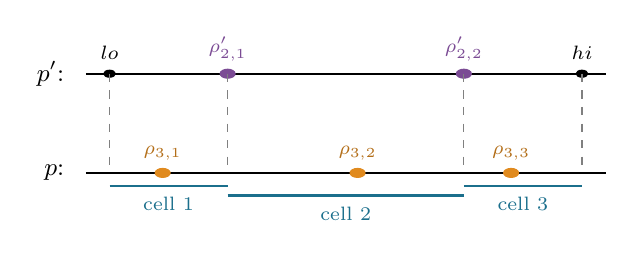
\begin{tikzpicture}[xscale=1.5,yscale=0.9]
  % line for p'
  \draw[thick] (-2.2,1.4) -- (2.2,1.4);
  \node[left,font=\small] at (-2.3,1.4) {$p'$:};
  \foreach \x/\n in {-1/{\rho_{2,1}'},1/{\rho_{2,2}'}} {
    \filldraw[ggplum] (\x,1.4) circle (1.8pt);
  }
  \node[ggplum,font=\scriptsize,above=1pt] at (-1,1.4) {$\rho'_{2,1}$};
  \node[ggplum,font=\scriptsize,above=1pt] at (1,1.4) {$\rho'_{2,2}$};
  % breakpoints
  \node[font=\scriptsize] at (-2,1.7) {$lo$};
  \node[font=\scriptsize] at (2,1.7) {$hi$};
  \filldraw (-2,1.4) circle (1.4pt); \filldraw (2,1.4) circle (1.4pt);
  % line for p with cells
  \draw[thick] (-2.2,0) -- (2.2,0);
  \node[left,font=\small] at (-2.3,0) {$p$:};
  \foreach \x in {-2,-1,1,2} \draw[gray,dashed] (\x,1.4) -- (\x,0);
  % cells brackets
  \draw[ggteal,thick] (-2,-0.18) -- (-1,-0.18); \node[ggteal,font=\scriptsize,below] at (-1.5,-0.2) {cell 1};
  \draw[ggteal,thick] (-1,-0.32) -- (1,-0.32);  \node[ggteal,font=\scriptsize,below] at (0,-0.34) {cell 2};
  \draw[ggteal,thick] (1,-0.18) -- (2,-0.18);   \node[ggteal,font=\scriptsize,below] at (1.5,-0.2) {cell 3};
  % virtual roots of p (R_d of each cell)
  \foreach \x in {-1.55,0.1,1.4} \filldraw[ggamber] (\x,0) circle (1.8pt);
  \node[ggamber!80!black,font=\scriptsize,above=1pt] at (-1.55,0) {$\rho_{3,1}$};
  \node[ggamber!80!black,font=\scriptsize,above=1pt] at (0.1,0) {$\rho_{3,2}$};
  \node[ggamber!80!black,font=\scriptsize,above=1pt] at (1.4,0) {$\rho_{3,3}$};
\end{tikzpicture}
\caption{The recursion, for $\deg p = 3$. The two virtual roots of $p'$ (plum) together with the
fences $lo,hi$ cut $[lo,hi]$ into three cells; on each cell $p'$ keeps a constant sign, so $\Rd_d$
returns one virtual root of $p$ (amber). Each $\rho_{3,j}$ lies in its own cell---this is what makes
them come out sorted and interlaced with the $\rho'_{2,j}$.}
\label{fig:construct}
\end{figure}

\section{Q3: where the formalization resists}\label{sec:q3}

\emph{A noncomputable choice, used honestly.} $\Rd_d$ is a \emph{chosen} minimiser, so \lean{R} is
\lean{noncomputable} and the development leans on \lean{Classical.choice}. That is sound and standard,
but it means the virtual roots are specified, not computed: the theorems are about \emph{a} minimiser,
and what makes them unambiguous is monotonicity. The two \emph{monotonicity bricks} shared with the
companion Budan--Fourier work---\lean{eval\_strictMonoOn\_of\_derivative\_pos} and its negative
twin---say that where $p'$ keeps a constant nonzero sign, $p$ is strictly monotone, so $|p|$ has a
\emph{single} well and the minimiser is unique. The formal development needs only existence and the
two facts \lean{R\_mem} / \lean{R\_eval\_eq\_zero}; uniqueness is what licenses the informal picture.

\emph{The breakpoints are a chain, and that is the crux.} Everything downstream rests on one
invariant: the augmented breakpoint list $lo::(\lean{vroots}\,lo\,hi\,p'\,)+\!\!+[hi]$ is
\emph{sorted}, and every virtual root lies in $[lo,hi]$. The two halves are mutually dependent---a
list is sorted only if its members are in range, and $\Rd_d$ lands in range only between sorted
breakpoints---so they are proved together, by a single induction down the derivative tower
(\lean{vroots\_chain\_mem}). The sortedness is the engine: because $\Rd_d(\mathrm{bps}[r],
\mathrm{bps}[r+1])$ lies in $[\mathrm{bps}[r],\mathrm{bps}[r+1]]$ and consecutive breakpoints are
ordered, consecutive virtual roots are ordered too (\lean{isChain\_zipWith\_R}). This is Rolle's
theorem in list form, and it is the part the machine would not let me wave away.

\emph{Indexing, and the small traps.} Turning ``each virtual root sits between its breakpoints'' into
a statement about \lean{getElem} required care that a hand proof hides. Rewriting a proof-carrying
indexed access (\lean{l[r]} drags a proof $r<\lean{l.length}$) is not a plain \lean{rw}; it goes
through \lean{simp} with the index lemmas, relying on proof irrelevance to reconcile the bounds. And
a destructuring \lean{rcases} on an equation $w=lo$ silently \emph{substitutes} $lo$ away in that
branch---a one-character fix (\lean{le\_rfl} for \lean{le\_refl lo}), but the kind of thing only a
kernel catches. These are not deep, but they are exactly the hand-waves a proof assistant refuses.

The bead handed on: the chain and the per-index localization are proved; \emph{what do they give, and
what stays out of reach for now?}

\section{Q4: what the certified theory gives}\label{sec:q4}

\emph{The Rolle interlacing.} The headline consequence is the interlacing of the virtual roots of $p$
with those of $p'$:
\begin{theorem}[Rolle interlacing of virtual roots; \lean{vroots\_interlacing}]\label{thm:interlace}
For $lo\le hi$ and each index $r$ in range,
\[
  \rho_{d,r}(p)\ \le\ \rho_{d-1,r}(p')\ \le\ \rho_{d,r+1}(p),
\]
i.e.\ \lean{(vroots lo hi p)[r] $\le$ (vroots lo hi (derivative p))[r] $\le$ (vroots lo hi p)[r+1]}.
\end{theorem}
\noindent The proof is two applications of the localization \lean{vroots\_getElem\_mem}---each virtual
root of $p$ lies between two breakpoints---together with the identity that the interior breakpoints
\emph{are} the virtual roots of $p'$. It is the discrete shadow of Rolle's theorem, and it places the
virtual-root family on the same footing as the interlacing families that run through the
real-rootedness literature---Newton's inequalities, the Heilmann--Lieb matching polynomial---where a
sequence and its derivative interleave. That this now holds for a family defined even when no real
roots exist is the point.

\emph{What it is the road to.} The interlacing is the structural half of the Budan--Fourier story.
The arithmetic half---that the number of virtual roots in a half-open interval $(a,b]$ equals the
sign-variation drop $\V(a)-\V(b)$ of the derivative tower~\cite{coste}---is the equality that the
classical Budan--Fourier inequality~\cite{bflean} only bounds. It is deliberately not proved here,
for an honest reason explained next: it fuses this construction with a second, independently recursive
one. The structural theory is complete; the count is the sequel.

\section{What a certified virtual-root theory enables}\label{sec:enables}

A machine-checked virtual-root family is the missing middle term between two things Mathlib already
has and one it does not. It has Descartes' rule (the coefficient sign count) and, in the companion
work, the Budan--Fourier \emph{inequality}; it does not have the object that would make that
inequality an equality. Virtual roots are that object. Downstream, they are the right input to a
certified real-root \emph{isolation} procedure in the line of Vincent, Collins and
Akritas~\cite{vincent,collinsakritas,akritas} and the sign-variation theory of
Basu--Pollack--Roy~\cite{bpr}---the count is exact, so a subdivision method reading
$\V(a)-\V(b)$ on each half has, in principle, a verified guarantee once the count theorem is added.
And because the family is defined for every polynomial, real-rooted or not, it connects the interval
methods to the algebra of the discriminant: a pair of virtual roots collides exactly when two real
roots are about to become complex, which is where the even Budan--Fourier surplus comes from. The
structural theory formalized here is the foundation all of that stands on.

\section{The building blocks}\label{sec:blocks}

Table~\ref{tab:results} gathers the load-bearing results, all \lean{sorry}-free in
\lean{VirtualRoots.lean}; Table~\ref{tab:metrics} measures the development. The dependency is short:
the monotonicity bricks give the existence and the two properties of $\Rd_d$; the combined induction
\lean{vroots\_chain\_mem} proves sortedness and range together; and the per-index localization gives
the interlacing.

\begin{table}[htbp]
  \centering\small
  \arrayrulecolor{ggteal}
  \begin{tabular}{@{}llc@{}}
    \toprule
    \rowcolor{ggteal}
    \textcolor{white}{\textbf{Lean name}} & \textcolor{white}{\textbf{Statement}} & \textcolor{white}{\textbf{Status}} \\
    \midrule
    \rowcolor{ggband}
    \lean{R\_mem} & $\Rd_d(a,b,p)\in[a,b]$ & proved \\
    \lean{R\_eval\_eq\_zero\_of\_le\_zero\_le} & $p(a)\!\le\!0\!\le\!p(b)\Rightarrow p(\Rd_d(a,b,p))=0$ & proved \\
    \rowcolor{ggband}
    \lean{vroots\_length} & $\#\{\text{virtual roots of }p\}=\deg p$ & proved \\
    \lean{vroots\_isChain} & $lo::(\text{vroots }p)+\!\!+[hi]$ is sorted & proved \\
    \rowcolor{ggband}
    \lean{vroots\_subset\_Icc} & every virtual root lies in $[lo,hi]$ & proved \\
    \lean{vroots\_getElem\_mem} & $\mathrm{bps}[r]\le\rho_{d,r}(p)\le\mathrm{bps}[r{+}1]$ & proved \\
    \rowcolor{ggband}
    \lean{vroots\_interlacing} & $\rho_{d,r}(p)\le\rho_{d-1,r}(p')\le\rho_{d,r+1}(p)$ & proved \\
    \lean{card\_virtualRoot\_eq\_fourierVar} & $\#$ in $(a,b]=\V(a)-\V(b)$ & \textit{future (\S\ref{sec:boundary})} \\
    \bottomrule
  \end{tabular}
  \arrayrulecolor{black}
  \caption{The structural theory of virtual roots, all \lean{sorry}-free in \lean{VirtualRoots.lean}
  (Lean~4 / Mathlib). \lean{\#print axioms} on \lean{vroots\_interlacing}, \lean{vroots\_isChain},
  \lean{vroots\_getElem\_mem} reports only \lean{propext}, \lean{Classical.choice}, \lean{Quot.sound}.
  The last row is the named sequel, not part of this development.}
  \label{tab:results}
\end{table}

\begin{table}[htbp]
  \centering\small
  \arrayrulecolor{ggteal}
  \begin{tabular}{@{}lc@{}}
    \toprule
    \rowcolor{ggteal}
    \textcolor{white}{\textbf{Quantity}} & \textcolor{white}{\textbf{Value}} \\
    \midrule
    \rowcolor{ggband}
    Lean file & \lean{VirtualRoots.lean} \\
    Public theorems / definitions & 16 / 2 \\
    \rowcolor{ggband}
    Axioms (headline theorems) & \lean{propext}, \lean{Classical.choice}, \lean{Quot.sound} \\
    \lean{sorry} count & 0 \\
    \rowcolor{ggband}
    Toolchain & Lean~4 (godsil pin v4.30) over Mathlib \\
    \bottomrule
  \end{tabular}
  \arrayrulecolor{black}
  \caption{The development measured. Build: \lean{lake env lean VirtualRoots.lean}, exit~0.}
  \label{tab:metrics}
\end{table}

\section{The boundary of the contribution}\label{sec:boundary}

\emph{What is proved.} The structural theory of the $\Rd_d$ virtual roots, sorry-free: existence and
the count ($=\deg p$), that they are sorted and lie in the bracketing interval, that $\Rd_d$ returns
an actual root wherever $p$ changes sign, and the Rolle interlacing. These are the results of
Gonz\'alez-Vega--Lombardi--Mah\'e~\cite{glm} in their structural part.

\emph{What is not proved, and is the explicit sequel.} The exact Budan--Fourier count---that the
number of virtual roots in $(a,b]$ equals $\V(a)-\V(b)$~\cite{coste}---is \emph{not} formalized here.
It is not a missing line; it fuses two independent recursive constructions, the $\Rd_d$ minimiser of
this file and the sign-variation function \lean{fourierVar} of the Budan--Fourier
formalization~\cite{bflean}, and it is a development in its own right. Stating it as done would be
dishonest; it is named here as the next milestone, with the two endpoints (the interlacing here, the
inequality there) now both in place.

\emph{Scope of the construction.} The virtual roots are built on a fixed bracketing interval
$[lo,hi]$. The global object on all of $\R$ is recovered by taking $lo,hi$ beyond every root of the
derivative tower---a Cauchy bound, available in Mathlib (\lean{Polynomial.cauchyBound})---but that
extension is not carried out in this file.

\emph{Novelty.} To the best of my knowledge, virtual roots had not been formalized in any interactive
theorem prover before this. The claim rests on searches in June~2026 of: Mathlib (no virtual roots;
it has Descartes via \lean{Polynomial.signVariations}); the Coq \lean{mathcomp-real-closed} library
(actual roots and the Thom encoding, not virtual roots); the Isabelle AFP, whose \lean{Budan\_Fourier}
entry formalizes the inequality with multiplicity but not the virtual-root object; and HOL~Light
(Sturm and Descartes, not virtual roots). I make this claim at the level of the named object; I cannot
exclude an unpublished or differently-named development, and I would welcome a pointer.

\emph{Authorship.} The mathematics is classical, due to the authors cited. The formalization was
carried out with an AI assistant; the Lean kernel certifies the proofs, and the scope statements above
are mine.

\section{Reflective questions, for the next bead}\label{sec:questions}

A string of beads is meant to be continued. The worth of certifying this structural theory is
measured by what it lets one ask next, and ask more sharply. I close with the questions I would rather
carry forward than pretend to have settled---each a place where this work stops short, and each, I
think, a rung up from it rather than merely a loose end.

\begin{enumerate}\itemsep3pt
\item \emph{From two constructions to one count.} The headline equality
$\#\{\text{virtual roots in }(a,b]\}=\V(a)-\V(b)$ is the sequel, and there are two honest routes to it.
One \emph{bridges} the construction here---the $\Rd_d$ minimiser---to the sign-variation function
\lean{fourierVar} of the companion work~\cite{bflean}, turning that paper's
inequality~\cite{coste,glm} into an equality. The other \emph{defines} virtual roots a second time, as
the jumps of \lean{fourierVar}, where the count is almost definitional, and then proves the two
definitions agree. The interlacing proved here is free in the first definition; the count is free in
the second; \textbf{the equivalence of the two definitions is the real theorem}. Which route is
shorter in Lean is itself the question.
\item \emph{Continuity, the other half of their reason for being.} Virtual roots vary
\emph{continuously} with the coefficients---this is half of why Gonz\'alez-Vega--Lombardi--Mah\'e
introduced them~\cite{glm}---and continuity is not touched here. A formalization would have to make
$\Rd_d$, a chosen minimiser, depend continuously on $p$; the monotonicity bricks that pin the
minimiser down are the natural starting point, but the statement is genuinely analytic.
\item \emph{One interlacing, three faces.} The Rolle interlacing places virtual roots beside the
families that run through the real-rootedness literature: the roots of a polynomial and its
derivative (classical Rolle~\cite{rolle}), Newton's inequalities~\cite{newton}, and the
Heilmann--Lieb matching polynomial. Eisermann's abstract \emph{Sturm chains}~\cite{eisermann} already
axiomatize one such interlacing structure. Is there a single Lean notion of ``interlacing family''
that subsumes all of these---and where does the virtual-root family, defined even when no real roots
exist, sit inside it? That is the bead I would most like to carry forward.
\end{enumerate}

\begin{thebibliography}{99}\small
\bibitem{glm} L.~Gonz\'alez-Vega, H.~Lombardi, L.~Mah\'e, Virtual roots of real polynomials,
\emph{J.~Pure Appl.\ Algebra} \textbf{124} (1998), no.~1--3, 147--166.
\bibitem{coste} M.~Coste, T.~Lajous-Loaeza, H.~Lombardi, M.-F.~Roy, Generalized Budan--Fourier theorem
and virtual roots, \emph{J.~Complexity} \textbf{21} (2005), no.~4, 479--486.
\bibitem{descartes} R.~Descartes, \emph{La G\'eom\'etrie} (1637); the rule of signs bounds the number
of positive roots by the number of sign changes of the coefficients.
\bibitem{budan} F.~D.~Budan de Boislaurent, \emph{Nouvelle m\'ethode pour la r\'esolution des
\'equations num\'eriques}, Paris (1807; 2nd ed.\ 1822).
\bibitem{fourier} J.~Fourier, \emph{Analyse des \'equations d\'etermin\'ees}, Firmin Didot, Paris
(posthumous, 1831).
\bibitem{rolle} M.~Rolle, \emph{Trait\'e d'alg\`ebre} (1690); between two consecutive real roots of a
differentiable function lies a root of its derivative.
\bibitem{sturm} C.~Sturm, M\'emoire sur la r\'esolution des \'equations num\'eriques, \emph{M\'emoires
pr\'esent\'es par divers savants \`a l'Acad\'emie Royale des Sciences} \textbf{6} (1835) 271--318.
\bibitem{akritas} A.~G.~Akritas, Reflections on a pair of theorems by Budan and Fourier, \emph{Mathematics
Magazine} \textbf{55} (1982) 292--298.
\bibitem{collinsakritas} G.~E.~Collins, A.~G.~Akritas, Polynomial real root isolation using Descartes'
rule of signs, in \emph{Proc.\ SYMSAC~'76}, ACM, 1976, 272--275.
\bibitem{vincent} A.~Alesina, M.~Galuzzi, A new proof of Vincent's theorem, \emph{L'Enseignement
Math\'ematique} \textbf{44} (1998) 219--256.
\bibitem{bpr} S.~Basu, R.~Pollack, M.-F.~Roy, \emph{Algorithms in Real Algebraic Geometry}, 2nd ed.,
Algorithms and Computation in Mathematics \textbf{10}, Springer, 2006 (sign-variation theory, Ch.~2,
and virtual roots).
\bibitem{eisermann} M.~Eisermann, The fundamental theorem of algebra made effective: an elementary
real-algebraic proof via Sturm chains, \emph{Amer.\ Math.\ Monthly} \textbf{119} (2012), no.~9,
715--752 (abstract ``Sturm chains'' and the Cauchy index).
\bibitem{liBF} W.~Li, L.~C.~Paulson, Counting polynomial roots in Isabelle/HOL: a formal proof of the
Budan--Fourier theorem, in \emph{Proc.\ CPP~2019}, ACM, 2019, 52--64; Archive of Formal Proofs entry
``The Budan--Fourier Theorem'' (W.~Li, 2018), \url{https://isa-afp.org/entries/Budan_Fourier.html}
(formalizes the inequality with multiplicity, not the virtual-root object).
\bibitem{cohen} C.~Cohen, Construction of real algebraic numbers in Coq, in \emph{Interactive Theorem
Proving (ITP 2012)}, LNCS \textbf{7406}, Springer, 2012, 67--82 (basis of \lean{mathcomp-real-closed}:
actual roots and the Thom encoding, not virtual roots).
\bibitem{eberl} M.~Eberl, Sturm's Theorem, \emph{Archive of Formal Proofs} (2014),
\url{https://isa-afp.org/entries/Sturm_Sequences.html}.
\bibitem{mathlib} The mathlib Community, The Lean mathematical library, in \emph{Certified Programs and
Proofs (CPP 2020)}, ACM, 2020, 367--381.
\bibitem{lean4} L.~de Moura, S.~Ullrich, The Lean~4 theorem prover and programming language, in
\emph{Automated Deduction (CADE~28)}, LNCS \textbf{12699}, Springer, 2021, 625--635.
\bibitem{bflean} C.~Mar\'in, \emph{Counting with the Derivative Tower: the Budan--Fourier Theorem,
Machine-Checked in Lean~4} (2026, companion formalization; \lean{BudanFourier.lean}).
\bibitem{sturmlean} C.~Mar\'in, \emph{The Staircase of Signs: Sturm's Root-Counting Theorem,
Machine-Checked in Lean~4}, Zenodo, 2026, \texttt{doi:10.5281/zenodo.20707348}.
\bibitem{newton} C.~Mar\'in, \emph{The Inward Bow of a Real-Rooted Polynomial: Newton's Inequalities,
Machine-Checked in Lean~4}, Zenodo, 2026, \texttt{doi:10.5281/zenodo.20693064}.
\end{thebibliography}

\end{document}
